\documentclass[12pt]{article}

\usepackage{sbc-template}
\usepackage[brazil,american]{babel}
\usepackage[utf8]{inputenc}

\usepackage{graphicx}
\usepackage{url}
\usepackage{float}
\usepackage{listings}
\usepackage{color}
\usepackage{todonotes}
\usepackage{algorithmic}
\usepackage{algorithm}
\usepackage{hyperref}
\usepackage{indentfirst}
\usepackage{longtable}
\usepackage[inline]{enumitem}


\graphicspath{{./images/}}

\sloppy

\title{Laboratório 3\\- CPU MIPS Uniciclo –}

\author{GRUPO 6\\
	Dayanne Fernandes da Cunha, 13/0107191\\
	Lucas Mafra Chagas, 12/0126443\\
	Marcelo Giordano Martins Costa de Oliveira, 12/0037301\\
	Lucas Junior Ribas, 16/0052289\\
	Caio Nunes de Alencar Osório, 16/0115132\\
	Diego Vaz Fernandes, 16/0117925}

\address{Dep. Ciência da Computação -- Universidade de Brasília (UnB)\\
  CiC 116394 - OAC - Turma A
  \email{}
}

\begin{document}
\maketitle

\section{Objetivos}
\label{sec:Objetivos}

\begin{itemize}
\item Treinar o aluno com a linguagem de descrição de \textit{hardware} \textit{Verilog};
\item Familiarizar o aluno com a plataforma de desenvolvimento \textit{FPGA DE2} da \textit{Altera} e o software \textit{QUARTUS II};
\item Desenvolver a capacidade de análise e síntese de sistemas digitais usando uma Linguagem de Descrição de \textit{Hardware};
\item Apresentar ao aluno a implementação de uma \textit{CPU MIPS}.
\end{itemize}

\section{Ferramentas}
\label{sec:Materiais}

Todos os códigos escritos neste laboratório podem ser encontrados no repositório \url{https://github.com/Dayof/OAC172} do \textit{GitHub}.

\begin{itemize}
\item FPGA DE2 da Altera 
\item QUARTUS-II
\item Verilog HDL
\end{itemize}

\section{Exercícios - PARTE A}
\label{sec:exerciciosA}

\subsection{Exercício 4. Diagrama de fluxo para tratamento de exceção}
\label{subsec:dfluxoexc}

  O tratamento de exceção obtém a causa através de um registrador especial denominado "CAUSE" "\$13", o endereço de retorno é armazenado em outro registrador, o EPC "\$14" (exception progamer counter). Esses registradores especiais não fazem parte do conjunto de registradores de uso geral do MIPS, eles ficam em um local especial , chamado de coprocessor 0. As instruções usadas para acessar esses registradores são o mfc0 e o mtc0.
	  
\label
  -Abaixo você encontrara o diagrama completo da rotina de tratamento de exceção do MIPS, que foi baseada no systemv54.s . Os números conectam o diagrama, fechando o ciclo no número "12".

\begin{figure}[H]
	\flushleft
	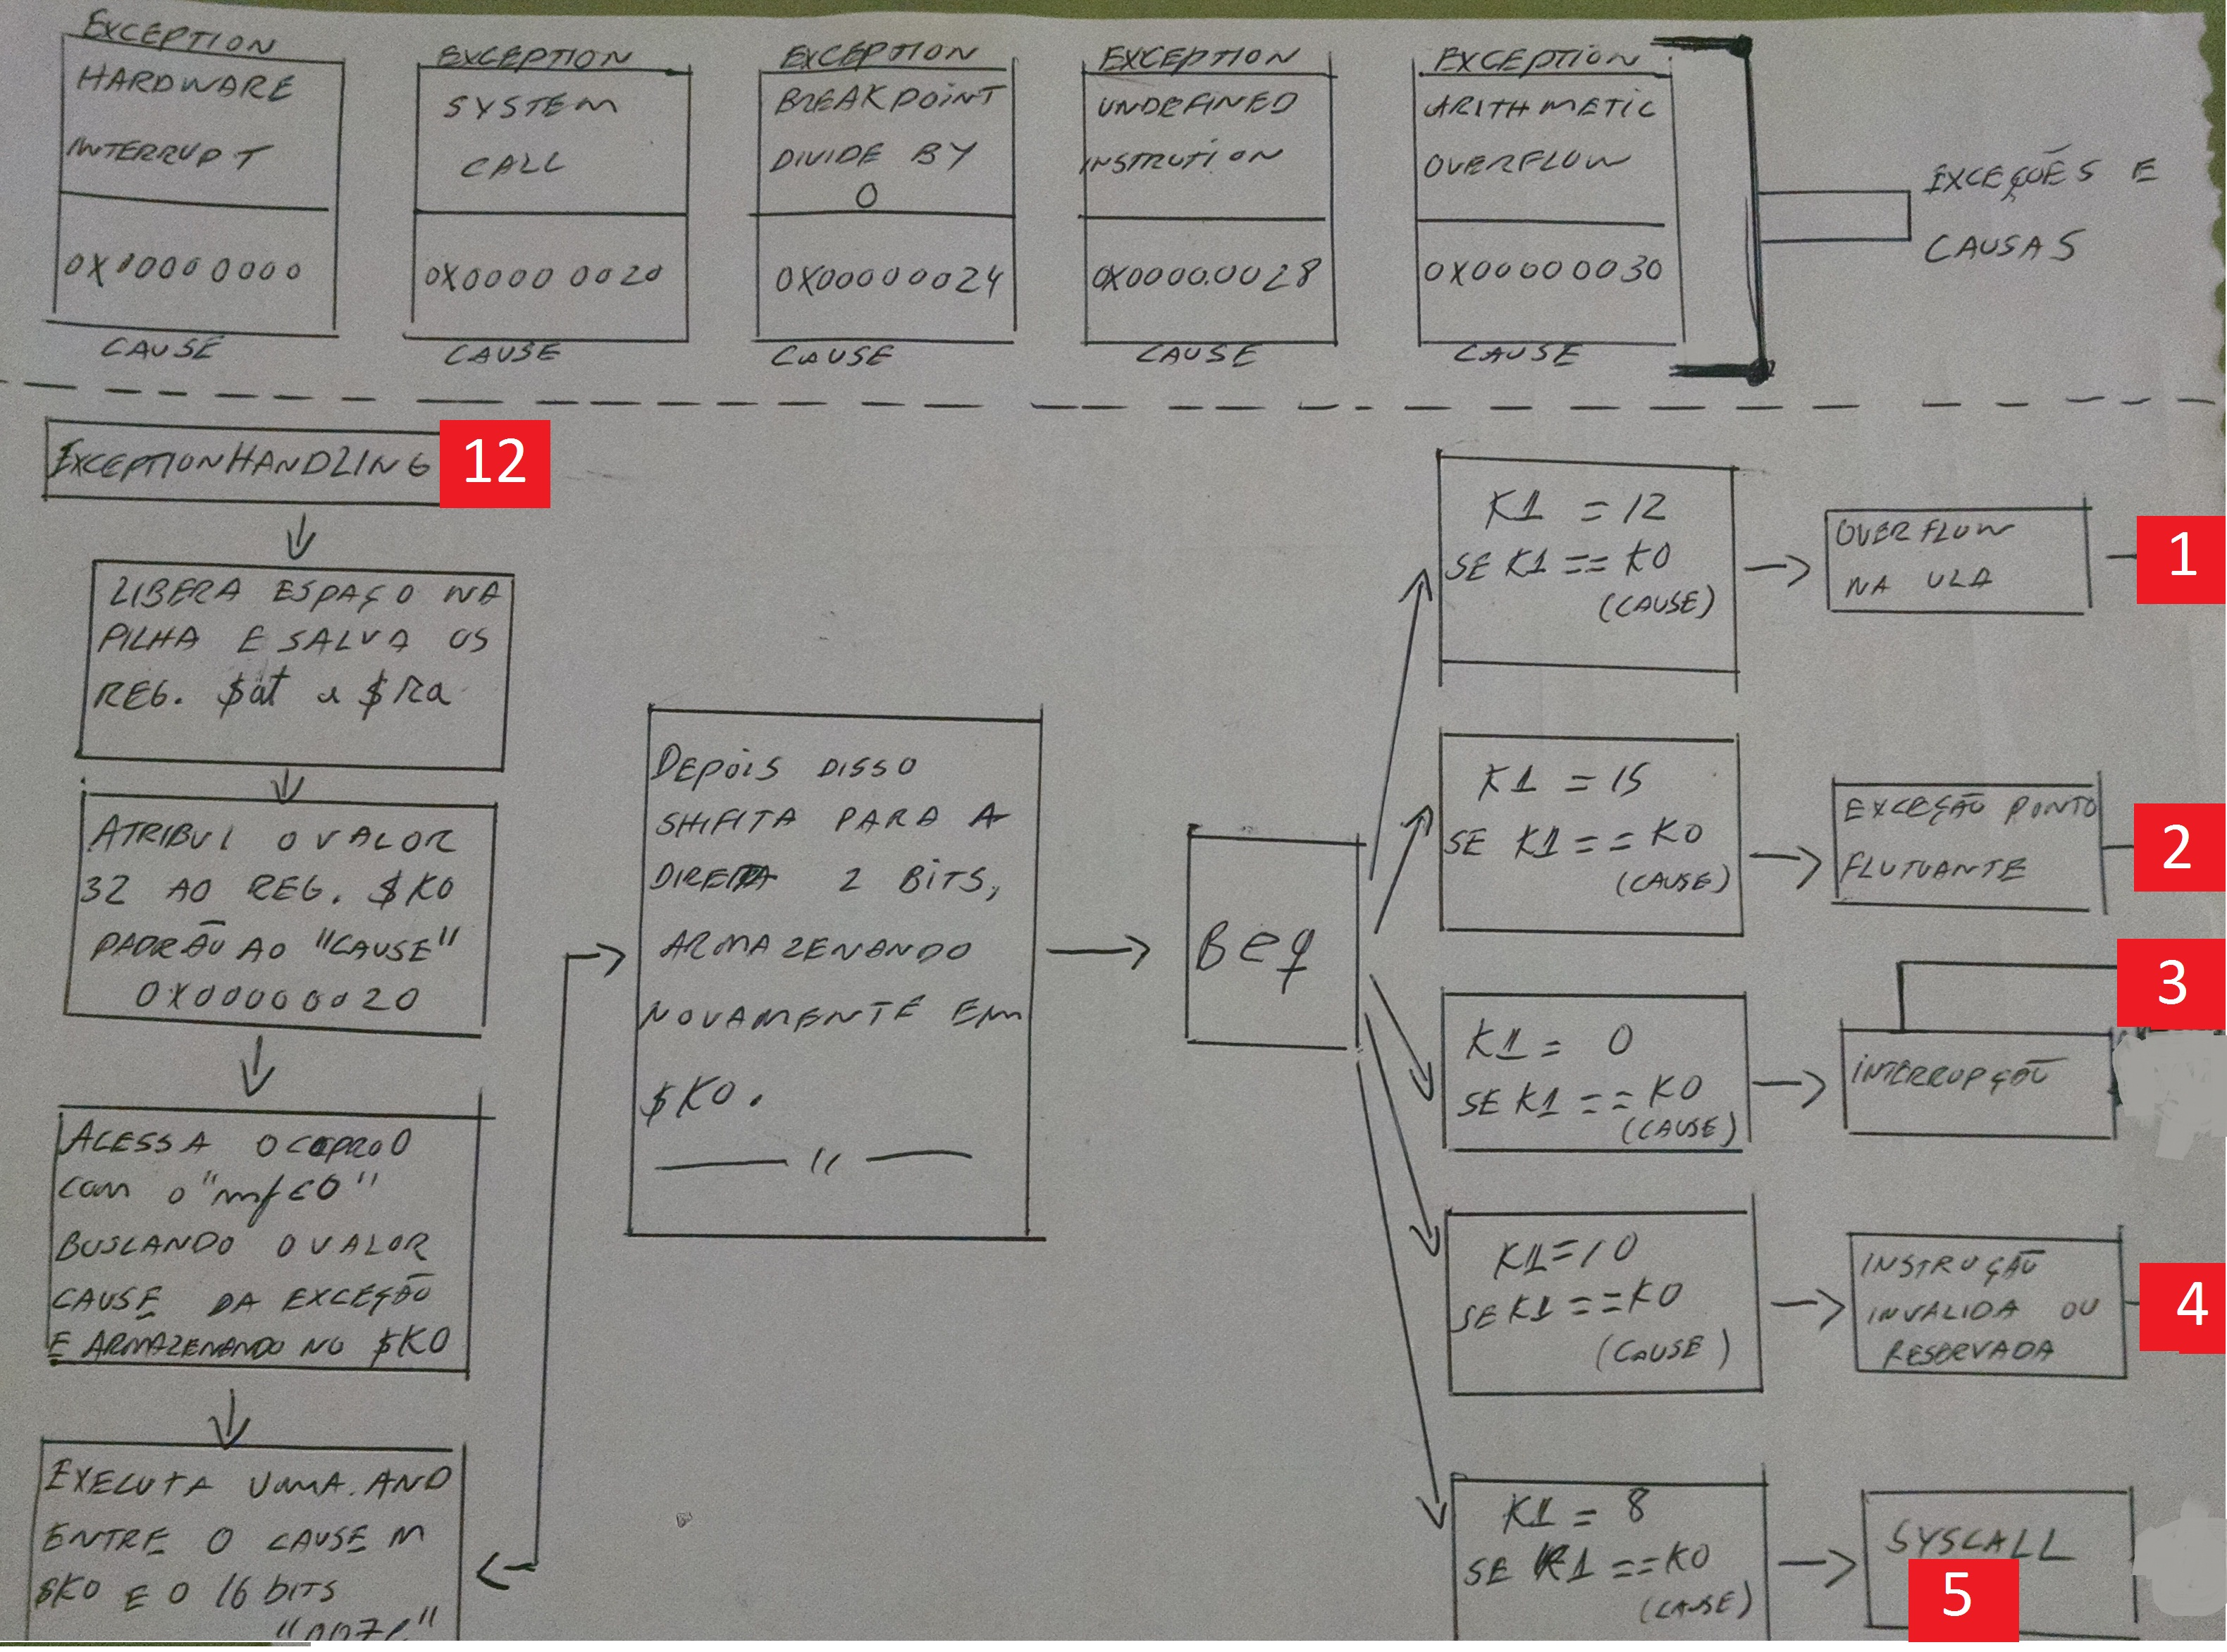
\includegraphics[width=1.1\textwidth]{imagens/1.jpg}
	\caption{ \textit{Parte 1}.}
	\label{fig:ex1st}
\end{figure}


\begin{figure}[H]
	\flushleft
	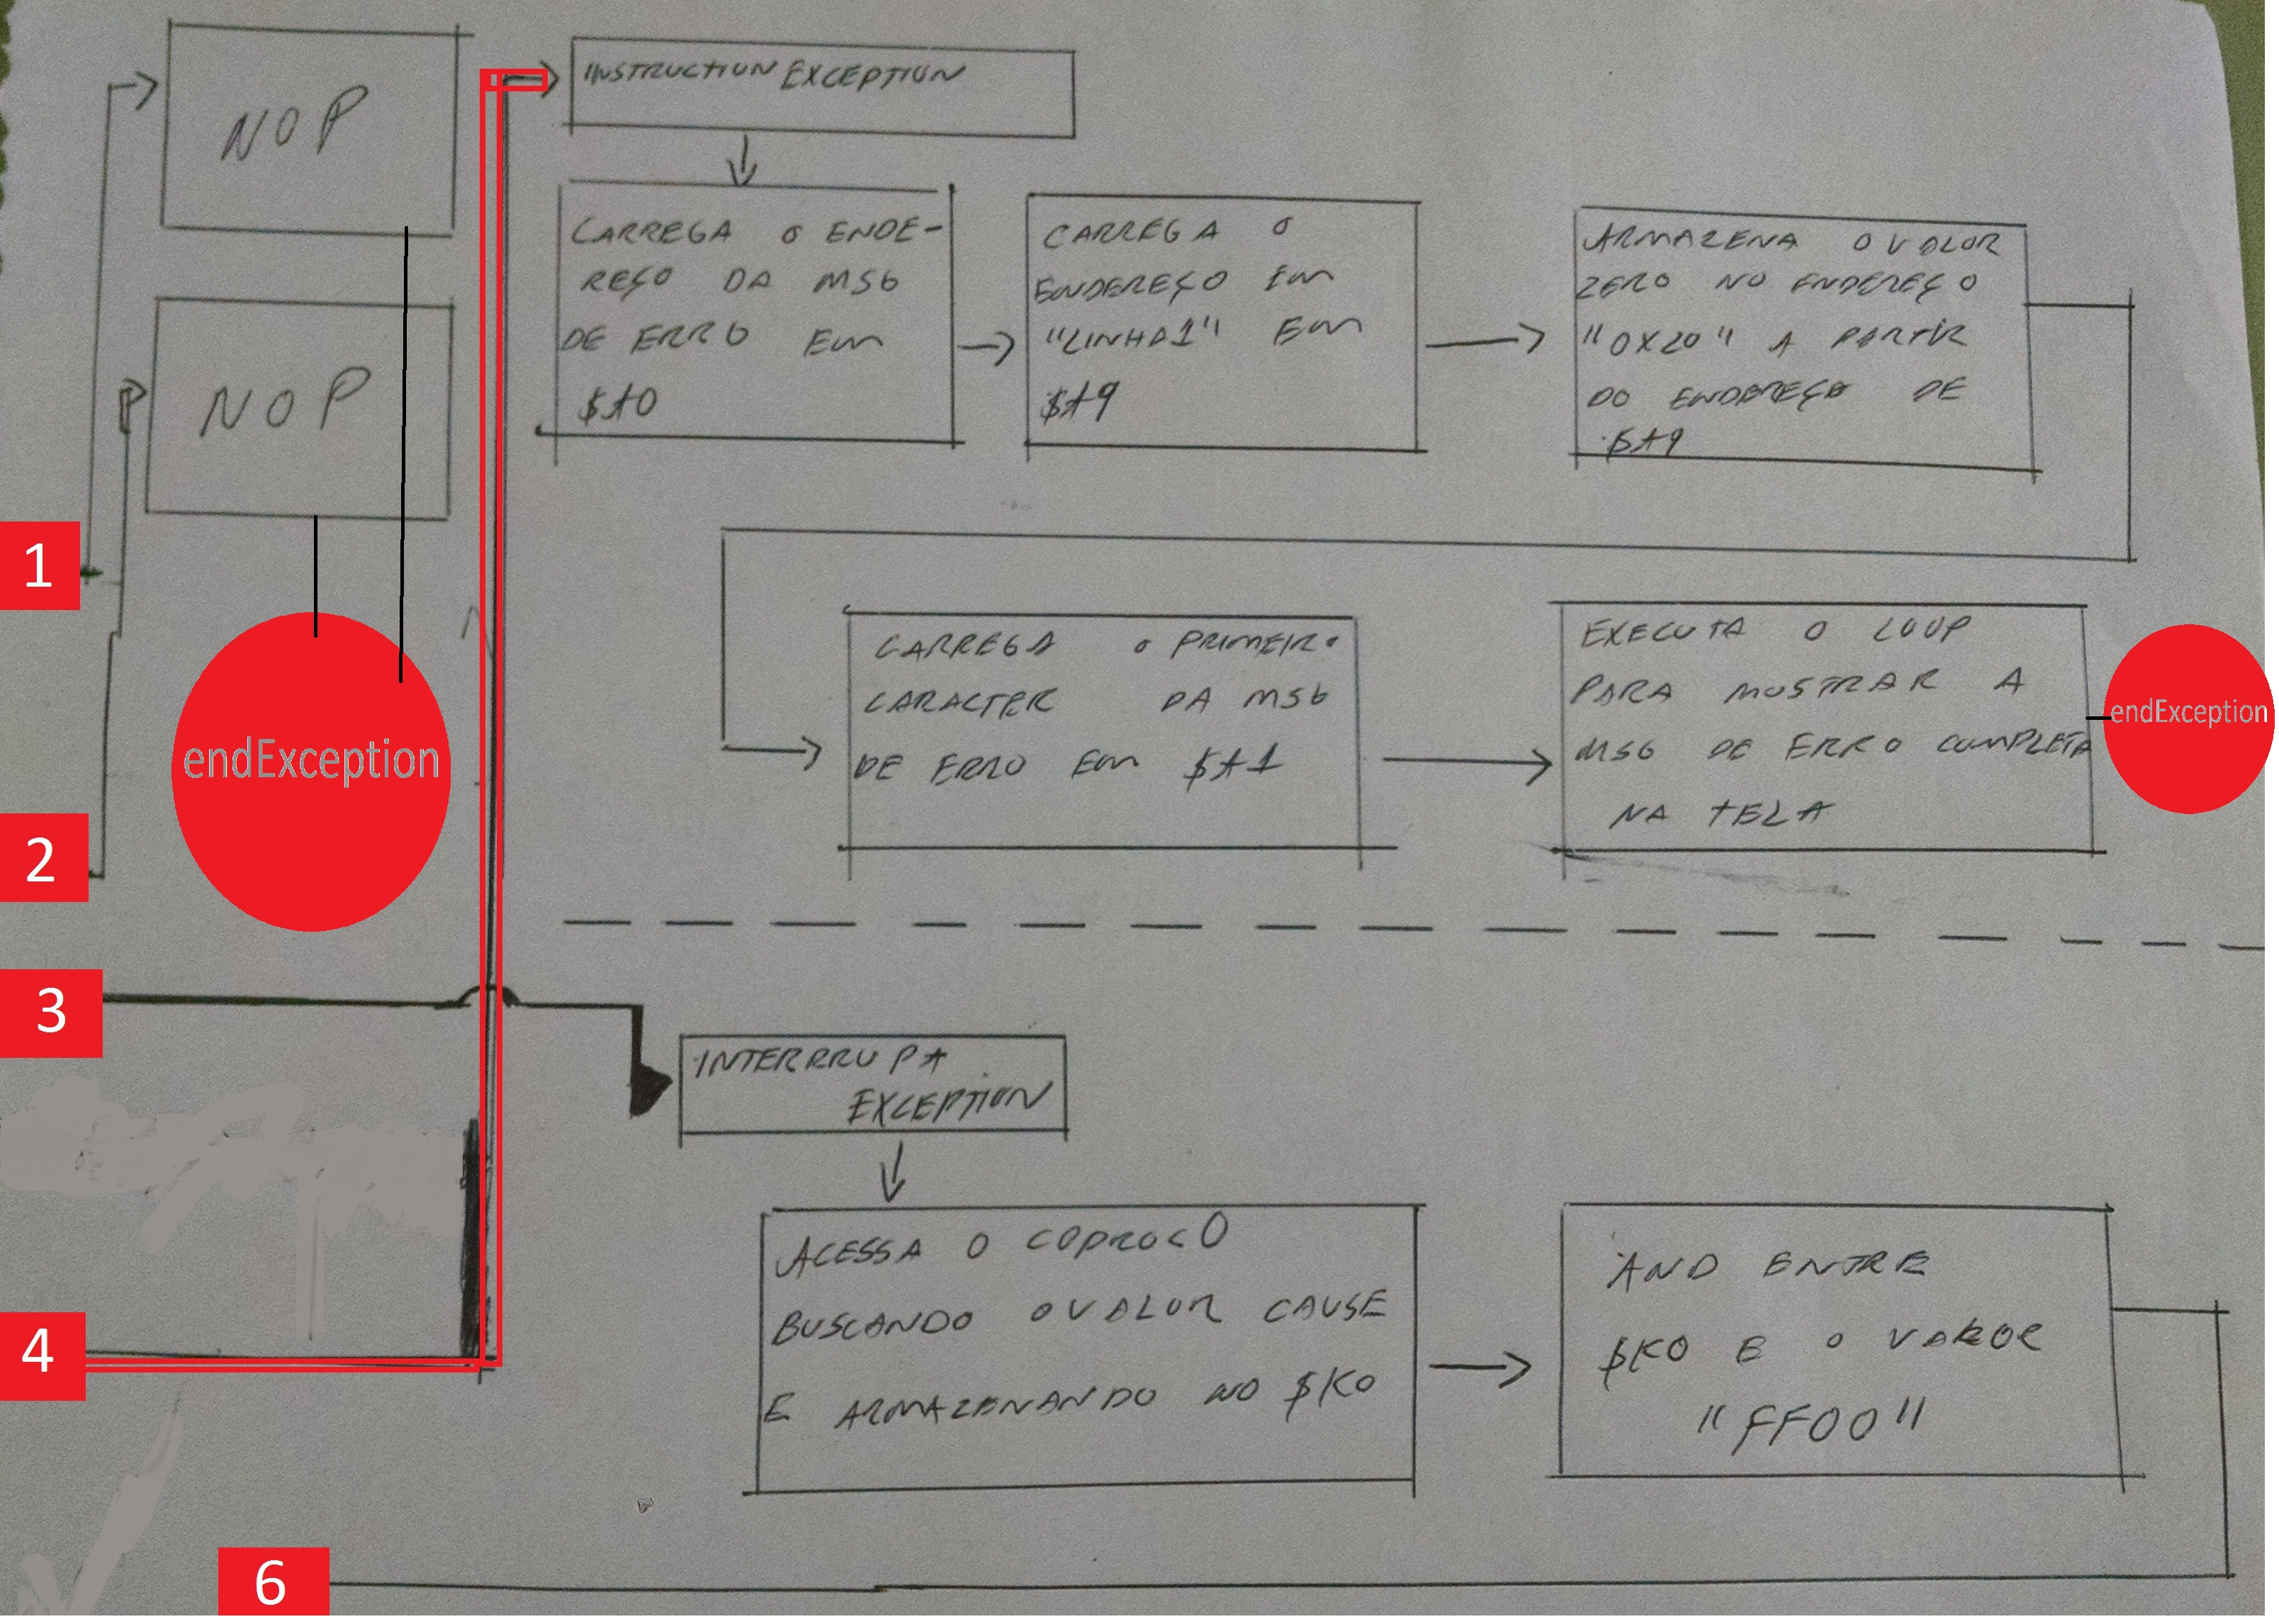
\includegraphics[width=1.1\textwidth]{imagens/2.jpg}
	\caption{ \textit{Parte 2}.}
	\label{fig:ex1st}
\end{figure}

\begin{figure}[H]
	\flushleft
	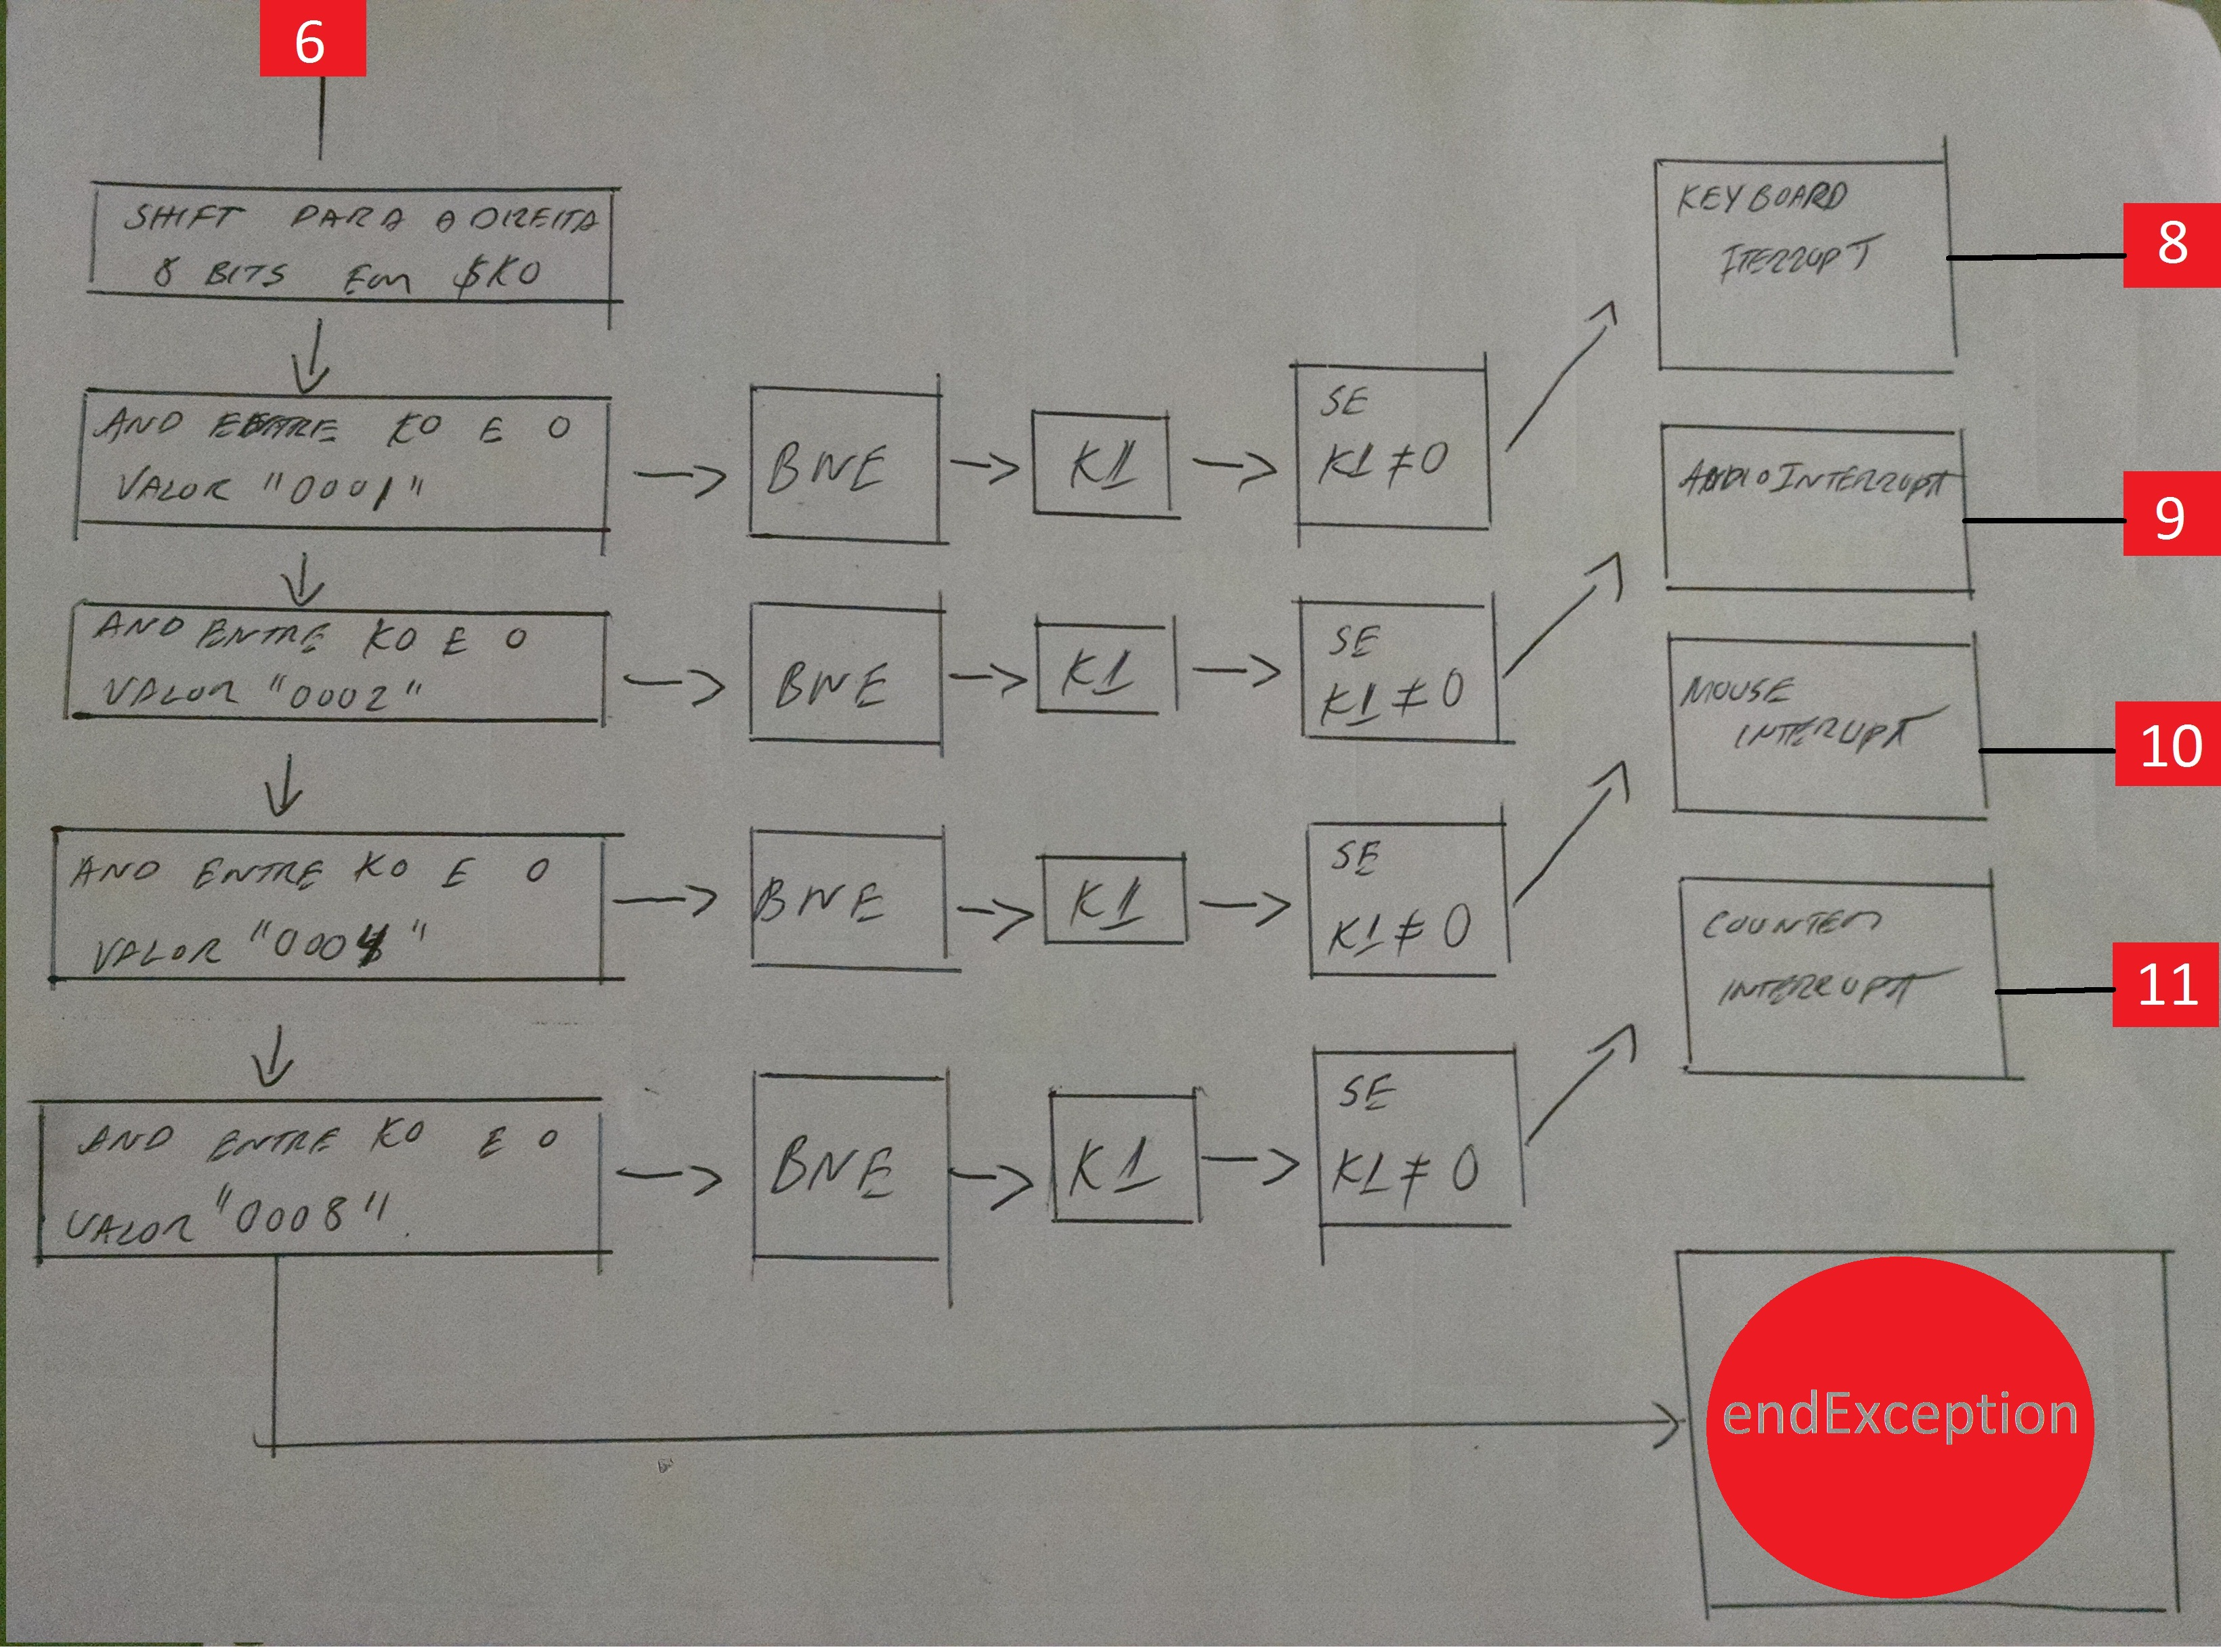
\includegraphics[scale=0.14]{imagens/5.jpg}
	\caption{ \textit{Parte 3}.}
	\label{fig:ex1st}
\end{figure}

\begin{figure}[H]
	\flushleft
	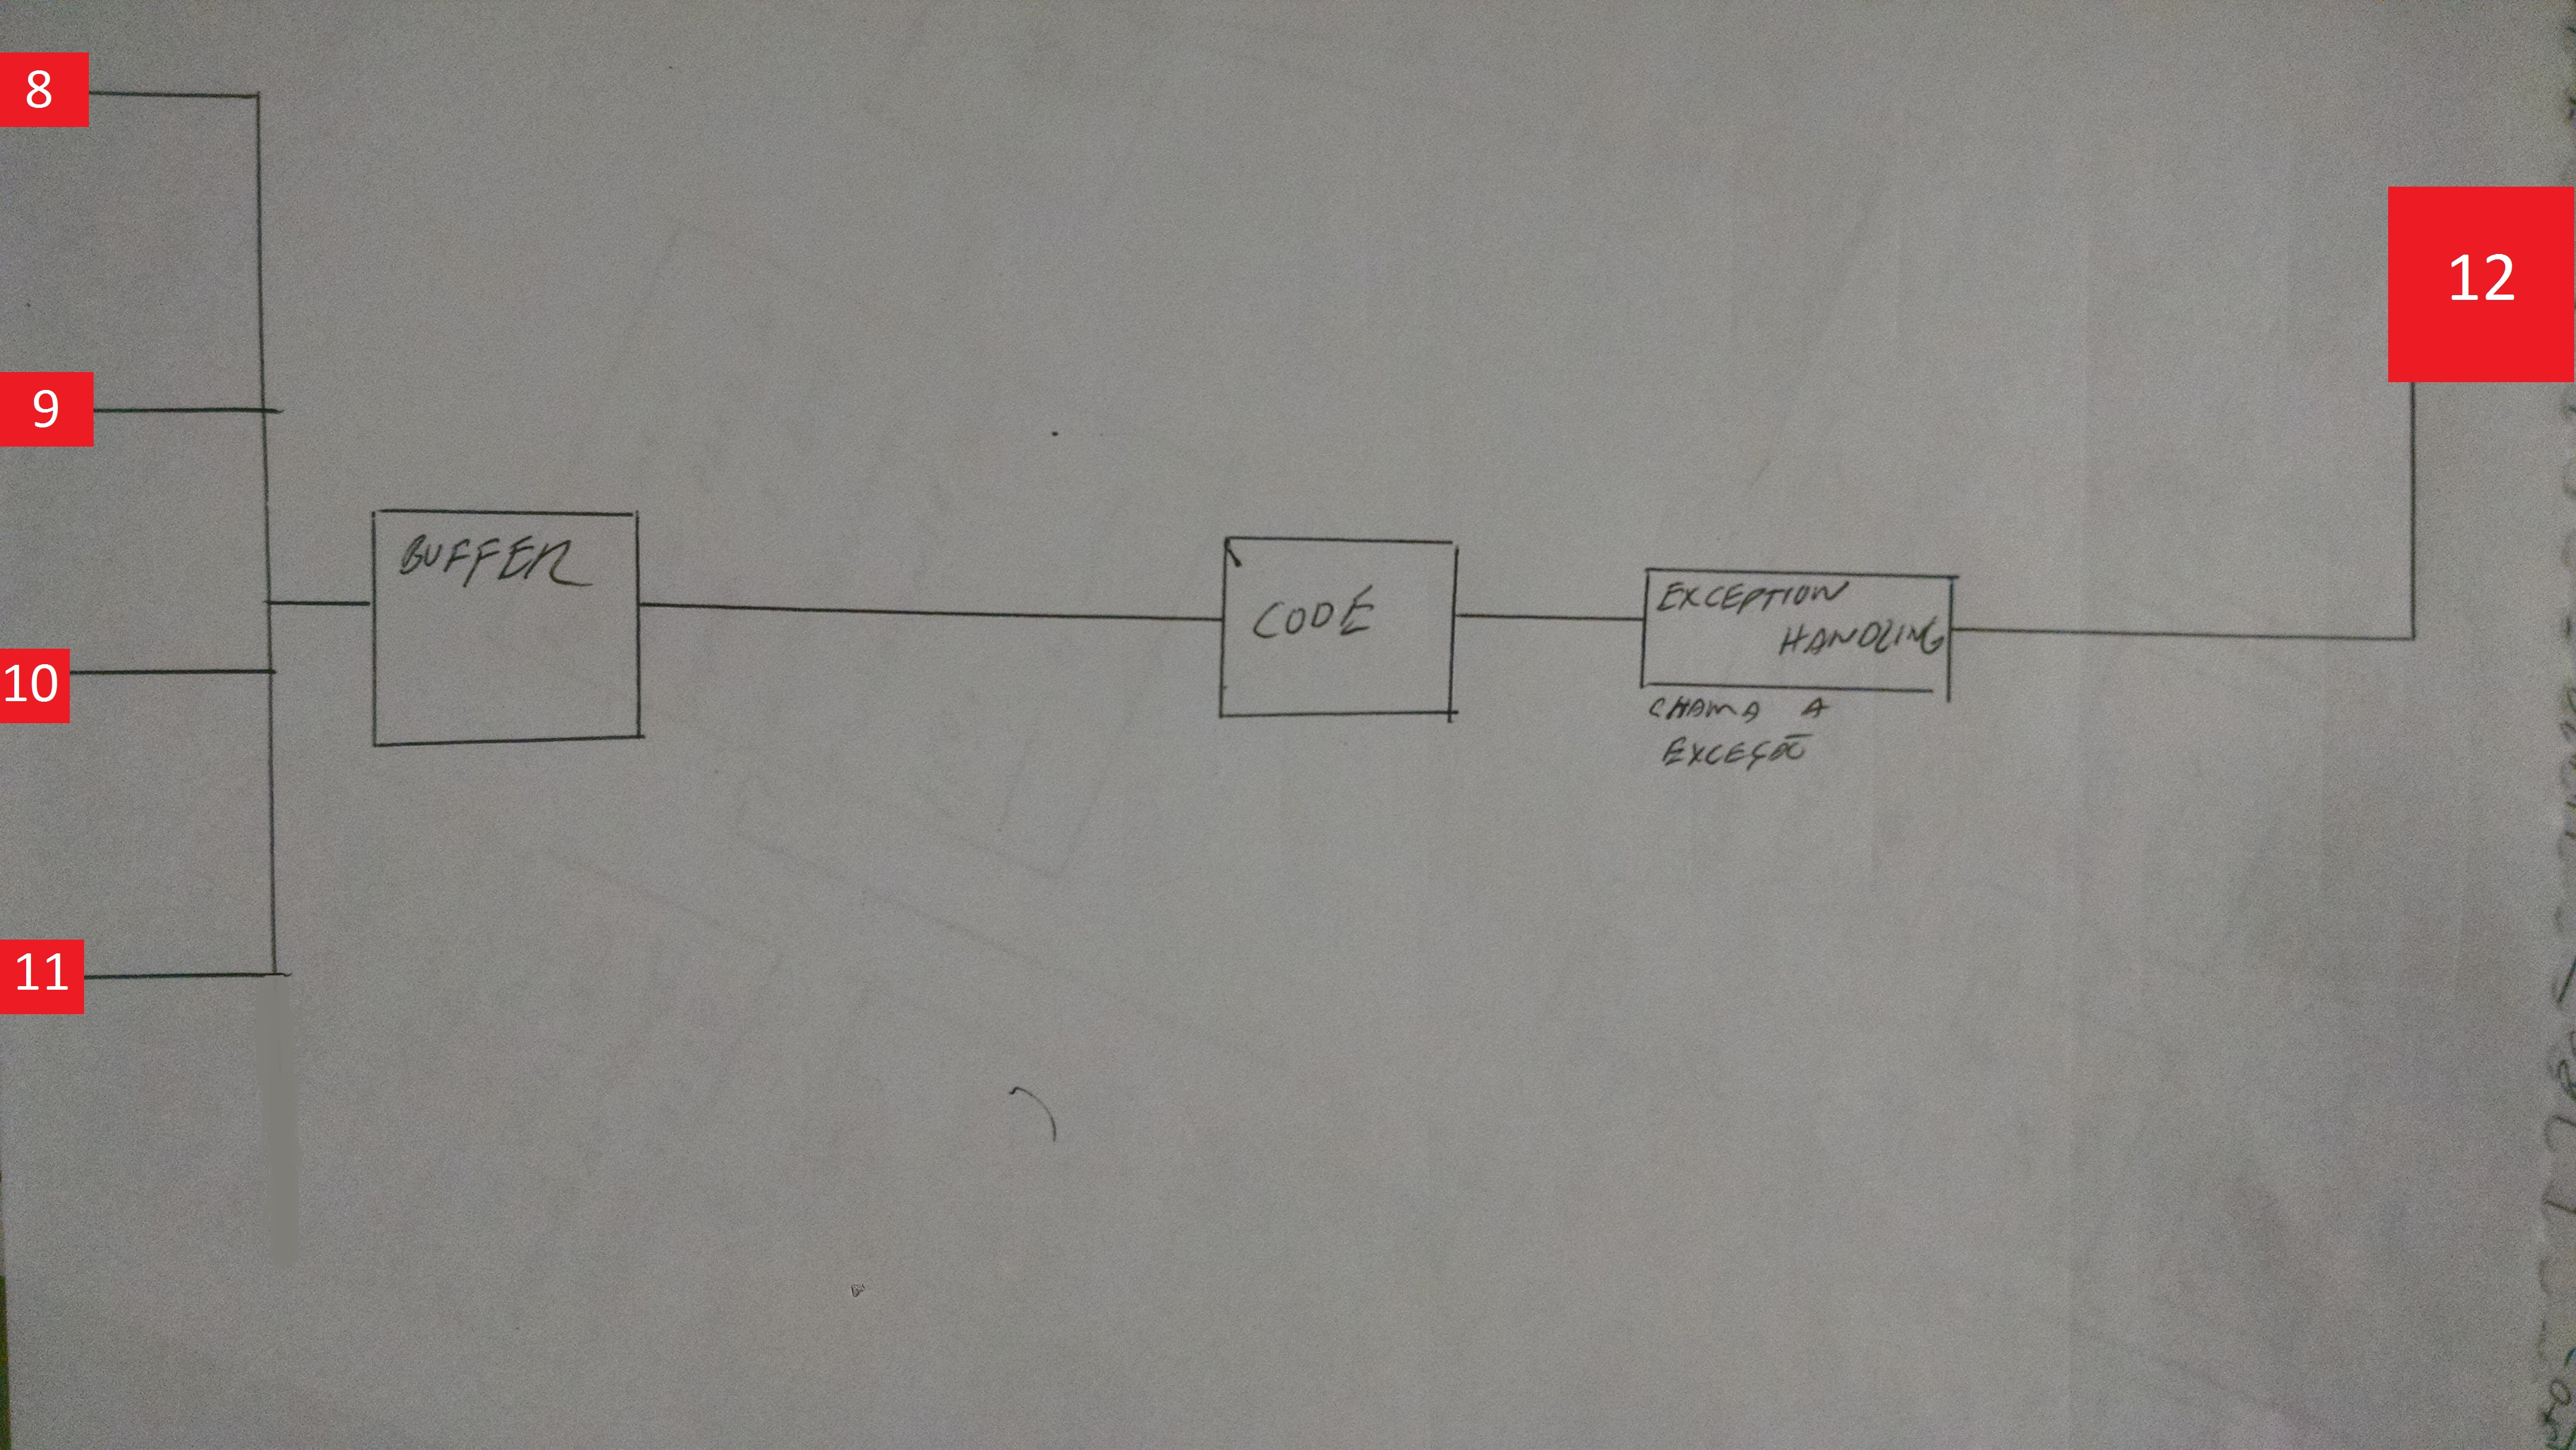
\includegraphics[scale=0.11]{imagens/6.jpg}
	\caption{ \textit{Parte 4}.}
	\label{fig:ex1st}
\end{figure}

\begin{figure}[H]
	\flushleft
	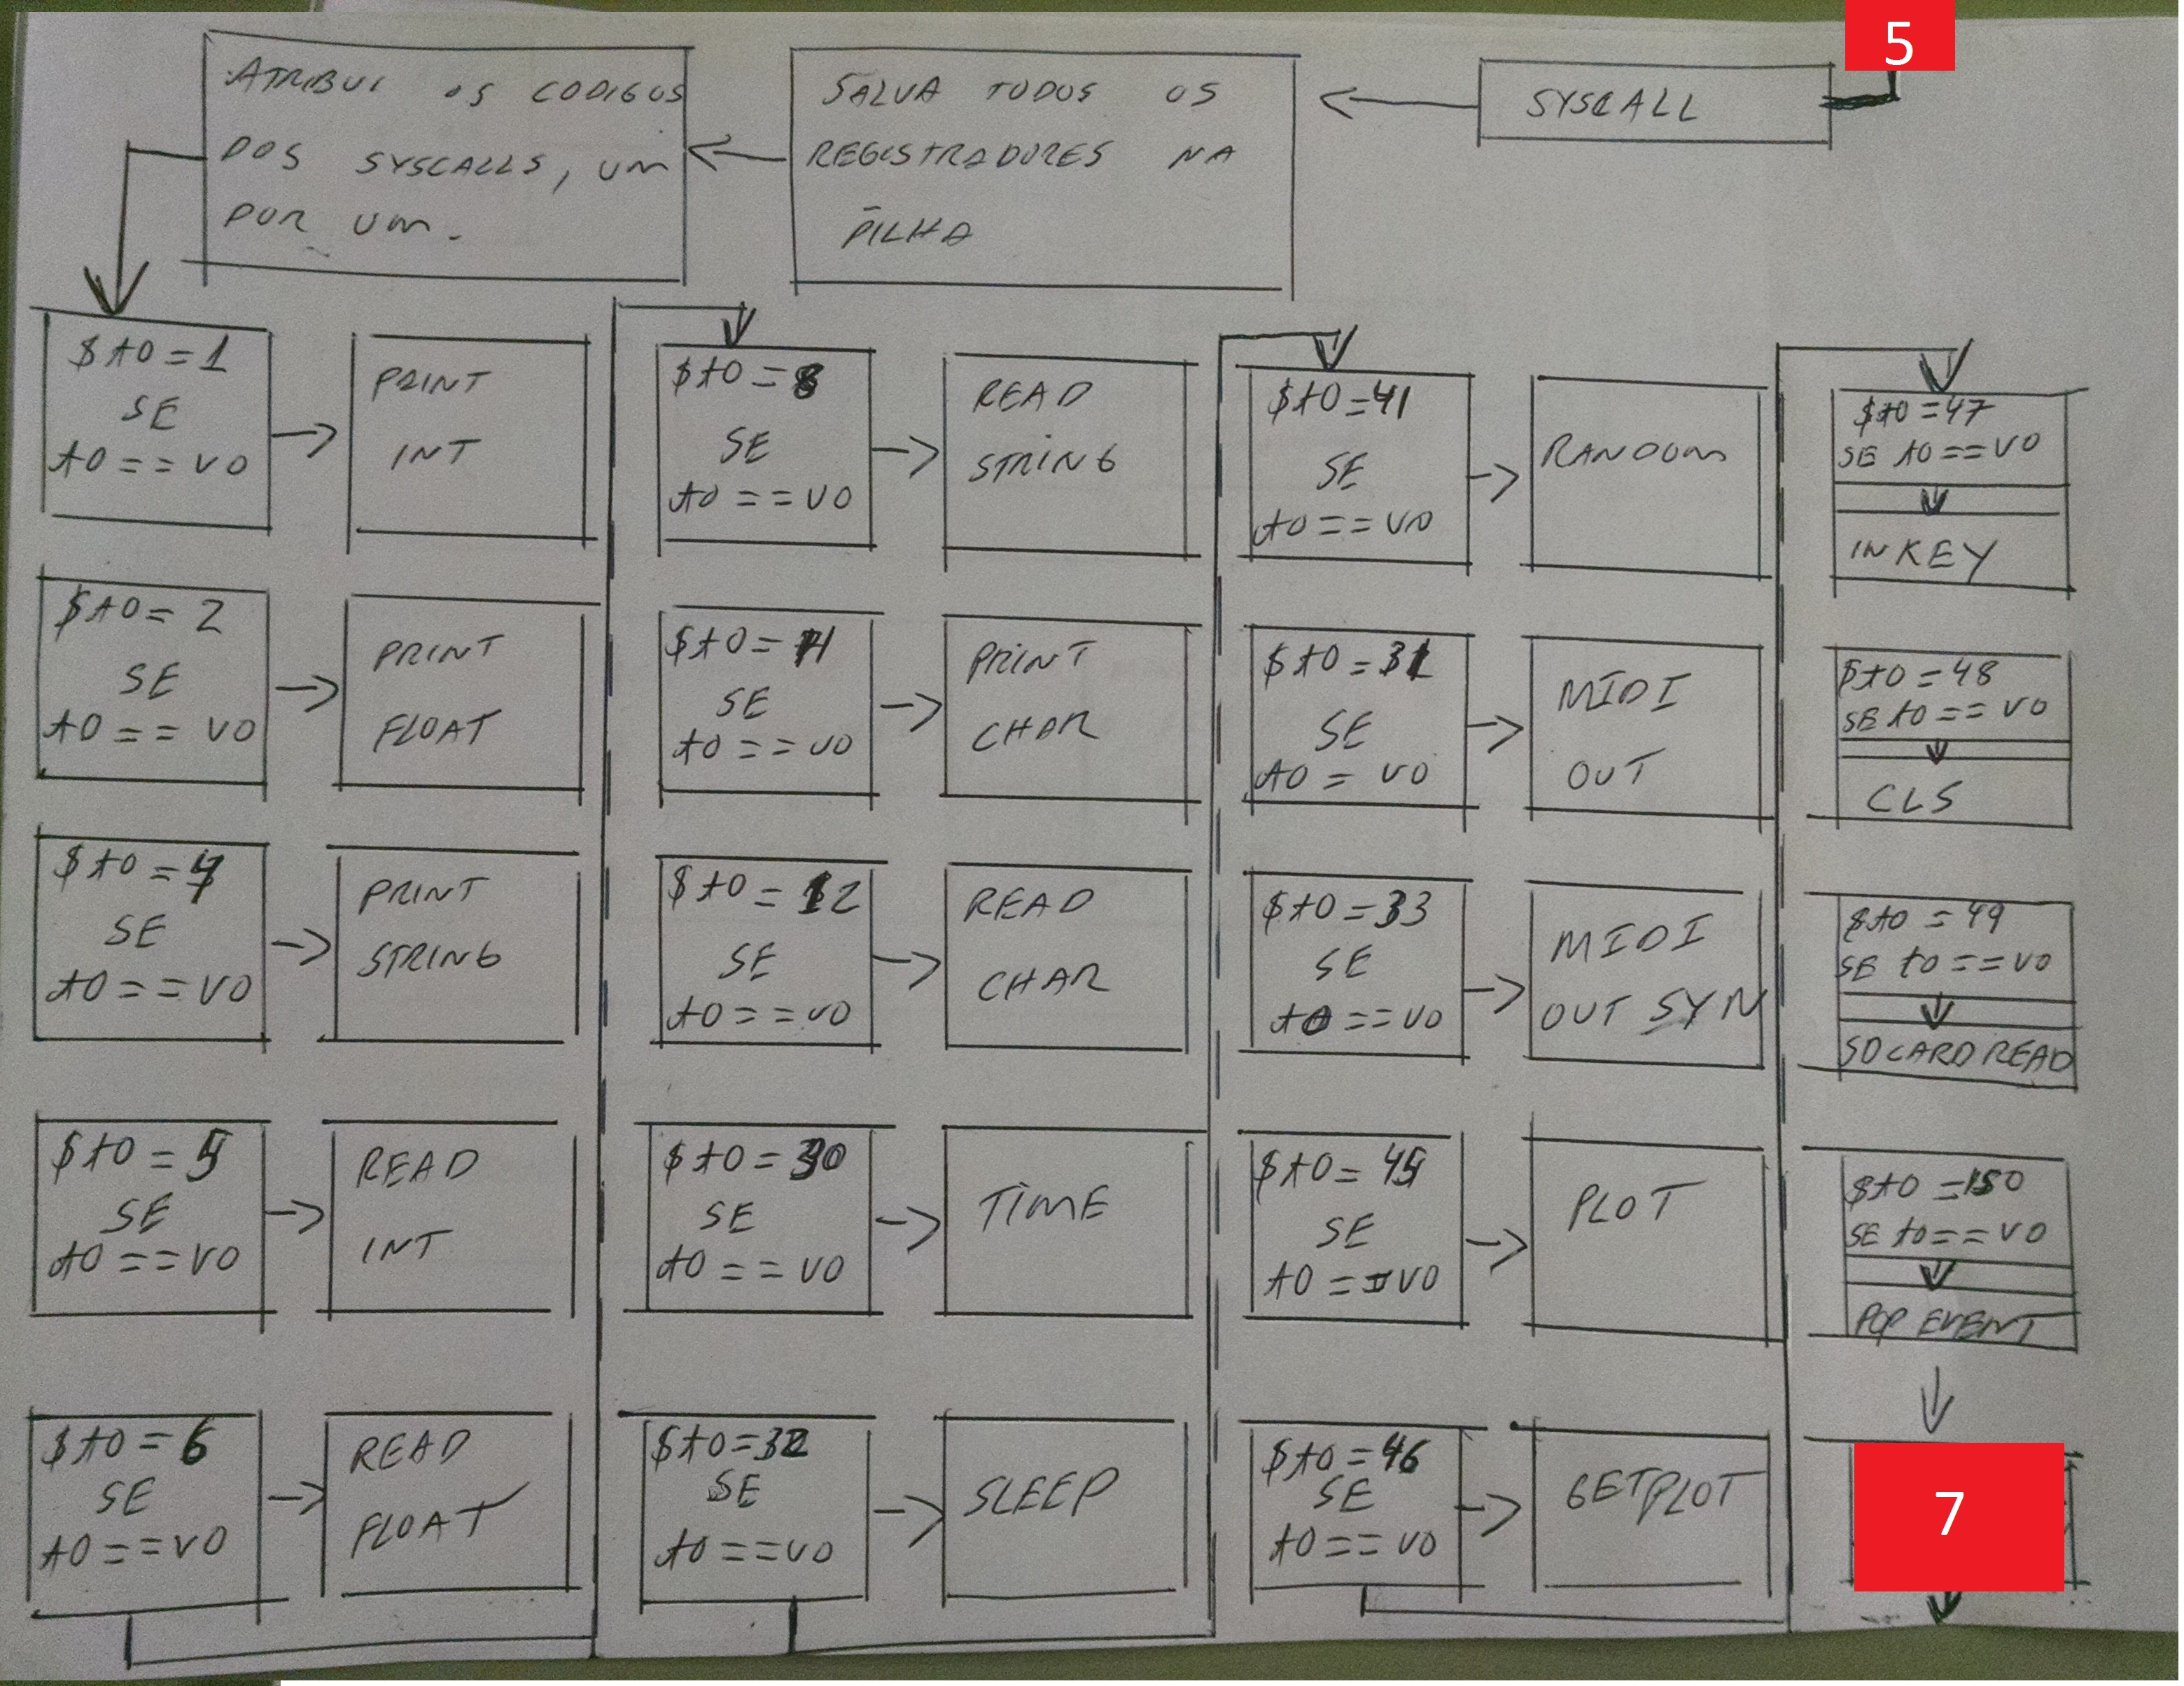
\includegraphics[scale=0.14]{imagens/3.jpg}
	\caption{ \textit{Parte 5}.}
	\label{fig:ex1st}
\end{figure}

\begin{figure}[H]
	\flushleft
	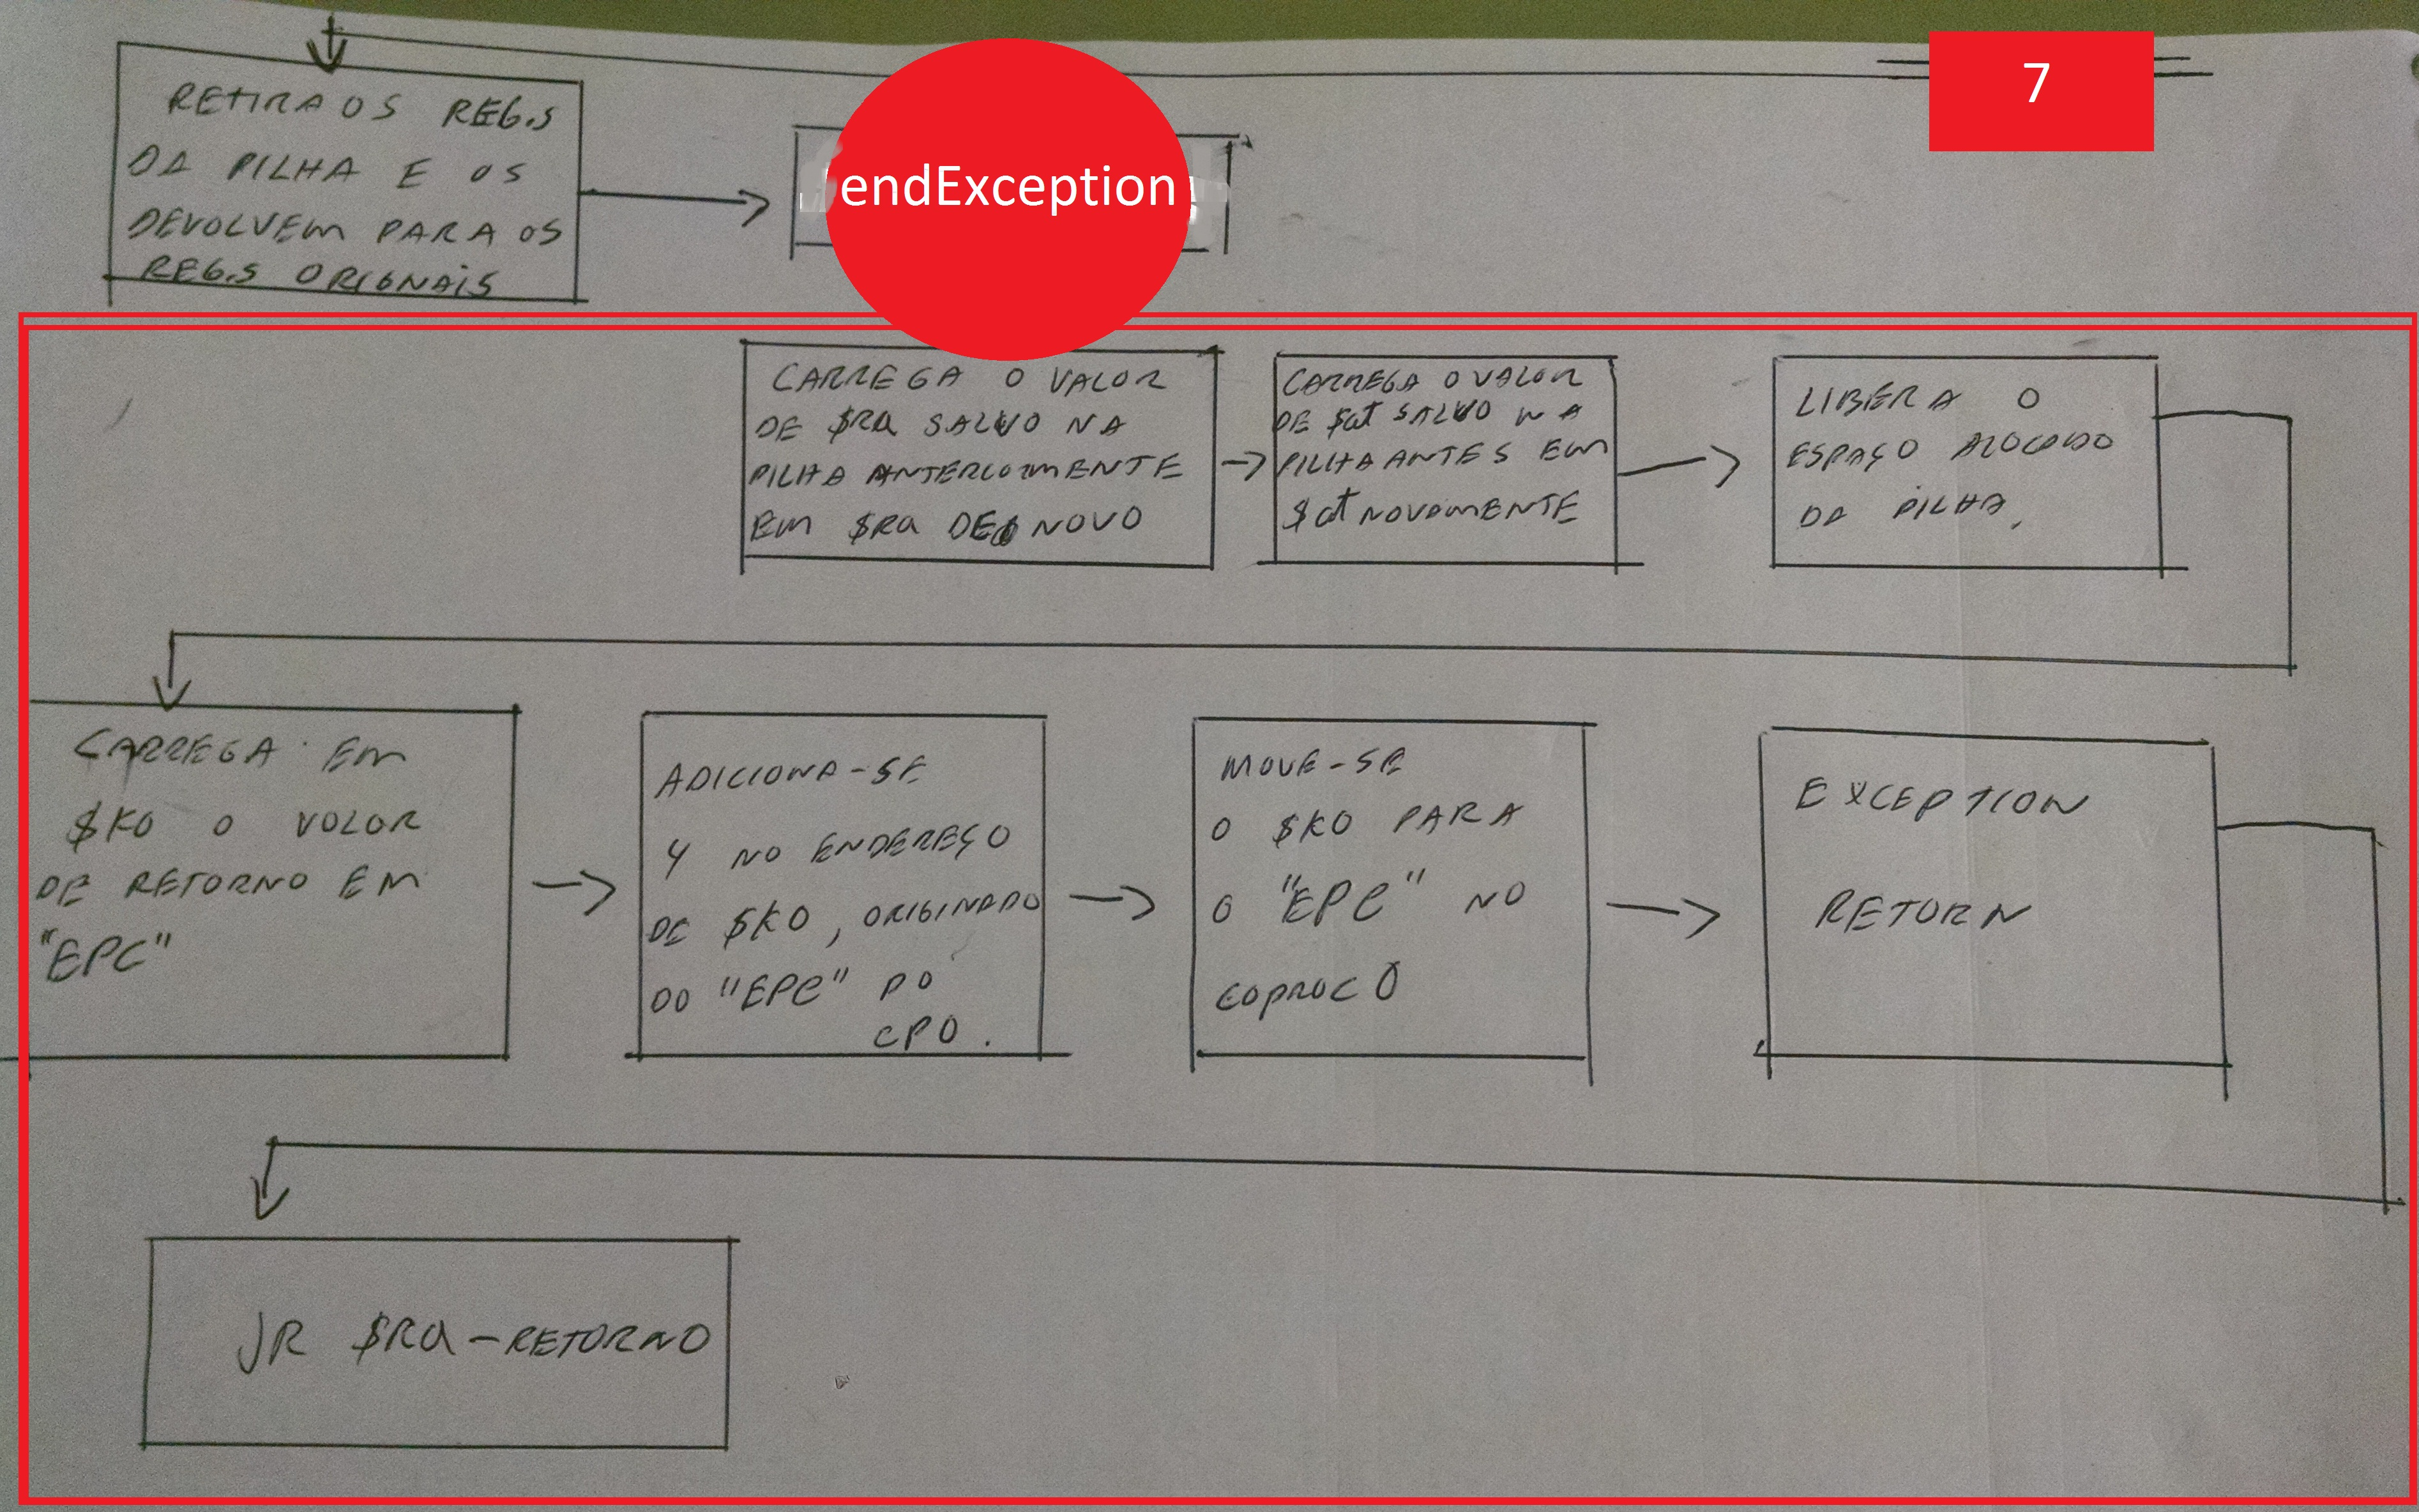
\includegraphics[scale=0.12]{imagens/4.jpg}
	\caption{ \textit{Parte 6}.}
	\label{fig:ex1st}
\end{figure}


\subsection{Exercício 5. Software de lançamento de bola de canhão na FPGA}
\label{subsec:canhao}

Abaixo, segue o vídeo demonstrativo da simulação do lançamento de bola de canhão executado na FPGA desenvolvido no laboratório 1:

\href{https://youtu.be/ipDxgTOtXDA}{Vídeo Demonstrativo}


\section{Exercícios - PARTE B}
\label{sec:exerciciosB}

\subsection{Exercício 7. Processador \textit{MIPS PUMv.5.1} UNICICLO}
\label{subsec:mips_uniciclo}

\begin{figure}[H]
	\flushleft
	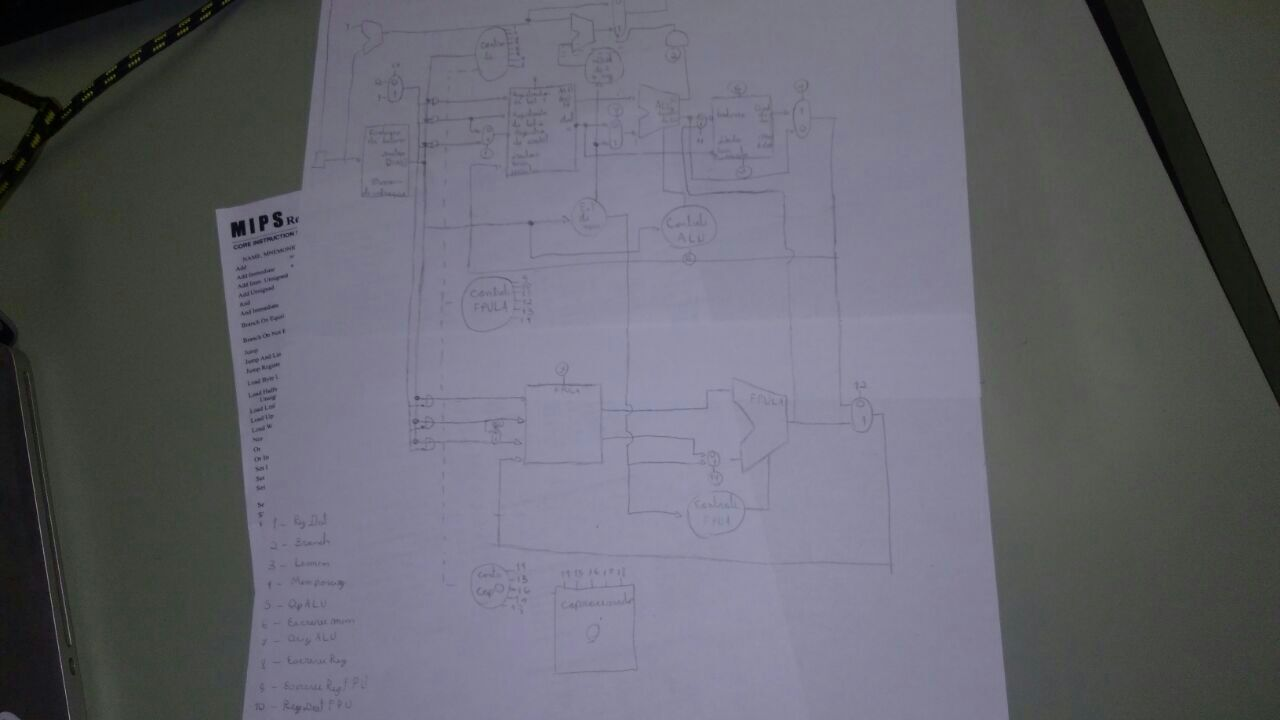
\includegraphics[scale=0.35]{imagens/diagrama.jpg}
	\caption{ \textit{Diagrama de blocos do Caminho de Dados}.}
	\label{fig:diagrama}
\end{figure}


\begin{longtable}{|c|c|c|c|c|c|c|}
		\hline
		 & oRegDst & oOrigALU & oMemforReg & oWriteReg & oReadMem & oWriteMem\\\hline
		 ADD/SUB & 01 & 00 & 000 & 1 & 0 & 0\\\hline	
		 ADDU/SUBU & 01 & 00 & 000 & 1 & 0 & 0\\\hline
		 SW/SH/SB & 00 & 01 & 000 & 0 & 0 & 1\\\hline
		 LBU/LHU & 00 & 01 & 110 & 1 & 1 & 0\\\hline
		 LB/LH & 00 & 01 & 110 & 1 & 1 & 0\\\hline
		 LW & 00 & 01 & 110 & 1 & 1 & 0\\\hline
		 BEQ & 00 & 00 & 000 & 0 & 0 & 0\\\hline	
		 BNE & 00 & 00 & 000 & 0 & 0 & 0\\\hline
		 JR & 00 & 00 & 000 & 0 & 0 & 0\\\hline
		 SYS & 00 & 00 & 000 & 0 & 0 & 0\\\hline
		 SLL/SRL/SRA & 01 & 00 & 000 & 1 & 0 & 0\\\hline
		 MFHI/MFLO & 01 & 00 & 000 & 1 & 0 & 0\\\hline
		 MTHI/MTLO & 01 & 00 & 000 & 1 & 0 & 0\\\hline
		 MUT/DIV & 01 & 00 & 000 & 1 & 0 & 0\\\hline
		 MUTU/DIVU & 01 & 00 & 000 & 1 & 0 & 0\\\hline
		 ADDU/SUBU & 01 & 00 & 000 & 1 & 0 & 0\\\hline
		 AND/OR & 01 & 00 & 000 & 1 & 0 & 0\\\hline
		 XNOR/NOR & 01 & 00 & 000 & 1 & 0 & 0\\\hline
		 SLT/SLTU & 01 & 00 & 000 & 1 & 0 & 0\\\hline
		 SLLV/SRLV & 01 & 00 & 000 & 1 & 0 & 0\\\hline
		 SRAV & 01 & 00 & 000 & 1 & 0 & 0\\\hline	
		 JMP & 01 & 00 & 000 & 0 & 0 & 0\\\hline
		 JAL & 10 & 11 & 010 & 1 & 0 & 0\\\hline
		 ADDI & 00 & 01 & 000 & 1 & 0 & 0\\\hline
		 ADDIU & 00 & 01 & 000 & 1 & 0 & 0\\\hline
		 SLTI/SLTIU & 00 & 01 & 000 & 1 & 0 & 0\\\hline
		 ANDI & 00 & 10 & 000 & 1 & 0 & 0\\\hline
		 XORI/ORI & 00 & 10 & 000 & 1 & 0 & 0\\\hline
		 LUI & 00 & 00 & 011 & 1 & 0 & 0\\\hline	
		 MTC & 00 & 00 & 000 & 0 & 0 & 0\\\hline
		 MFC & 00 & 00 & 100 & 1 & 0 & 0\\\hline
		 BC1-0 & 00 & 00 & 000 & 0 & 0 & 0\\\hline	
		 BC1-1 & 00 & 00 & 000 & 0 & 0 & 0\\\hline
		 ADDS/SUBS & 00 & 00 & 000 & 0 & 0 & 0\\\hline
		 MULS/DIVS & 00 & 00 & 000 & 0 & 0 & 0\\\hline
		 CVTSW & 00 & 00 & 000 & 0 & 0 & 0\\\hline	
		 SQRT & 00 & 00 & 000 & 0 & 0 & 0\\\hline
		 ABS/NEG & 00 & 00 & 000 & 0 & 0 & 0\\\hline
		 CVTWS & 00 & 00 & 000 & 0 & 0 & 0\\\hline
		 CEILWS & 00 & 00 & 000 & 0 & 0 & 0\\\hline
		 FLOORWS & 00 & 00 & 000 & 0 & 0 & 0\\\hline
		 ROUNDWS & 00 & 00 & 000 & 0 & 0 & 0\\\hline	
		 CEQ/CLT/CLE & 00 & 00 & 000 & 0 & 0 & 0\\\hline
		 MOV & 00 & 00 & 000 & 0 & 0 & 0\\\hline
		 SWC1 & 00 & 01 & 000 & 0 & 0 & 1\\\hline	
		 LWC1 & 00 & 01 & 000 & 0 & 1 & 0\\\hline
		 BGEZ & 00 & 11 & 000 & 0 & 0 & 0\\\hline	
		 BGEZAL & 10 & 11 & 010 & 1 & 0 & 0\\\hline
		 BLTZ & 00 & 11 & 000 & 0 & 0 & 0\\\hline
		 BLTZAL & 11 & 11 & 010 & 1 & 0 & 0\\\hline
		 BLEZ & 00 & 11 & 000 & 0 & 0 & 0\\\hline
		 BGTZ & 00 & 11 & 000 & 0 & 0 & 0\\\hline
		 MFC & 00 & 00 & 101 & 1 & 0 & 0\\\hline	
		 MTC & 00 & 00 & 000 & 0 & 0 & 0\\\hline
		 ERET & 00 & 00 & 000 & 0 & 0 & 0\\\hline			
	\caption{Tabela verdade das operações da ISA.}
	\label{tab:req21}
\end{longtable}

\begin{longtable}{|c|c|c|c|c|c|c|}
		\hline
		& oOrigPC & oOpALU & oWRegFPU & oRDFPU & oFPUpMem & oDRFPU\\\hline
		ADD/SUB & 000 & 11 & 0 & 00 & 00 & 00\\\hline	
		ADDU/SUBU & 000 & 11 & 0 & 00 & 00 & 00\\\hline
		SW/SH/SB & 000 & 00 & 0 & 00 & 10 & 00\\\hline
		LBU/LHU & 000 & 00 & 0 & 00 & 00 & 00\\\hline
		LB/LH & 000 & 00 & 0 & 00 & 00 & 00\\\hline
		LW & 000 & 00 & 0 & 00 & 00 & 00\\\hline
		BEQ & 001 & 01 & 0 & 00 & 00 & 00\\\hline	
		BNE & 101 & 01 & 0 & 00 & 00 & 00\\\hline
		JR & 011 & 00 & 0 & 00 & 00 & 00\\\hline
		SYS & 100 & 00 & 0 & 00 & 00 & 00\\\hline
		SLL/SRL/SRA & 000 & 10 & 0 & 00 & 00 & 00\\\hline
		MFHI/MFLO & 000 & 10 & 0 & 00 & 00 & 00\\\hline
		MTHI/MTLO & 000 & 10 & 0 & 00 & 00 & 00\\\hline
		MUT/DIV & 000 & 10 & 0 & 00 & 00 & 00\\\hline
		MUTU/DIVU & 000 & 10 & 0 & 00 & 00 & 00\\\hline
		ADDU/SUBU & 000 & 10 & 0 & 00 & 00 & 00\\\hline
		AND/OR & 000 & 10 & 0 & 00 & 00 & 00\\\hline
		XNOR/NOR & 000 & 10 & 0 & 00 & 00 & 00\\\hline
		SLT/SLTU & 000 & 10 & 0 & 00 & 00 & 00\\\hline
		SLLV/SRLV & 000 & 10 & 0 & 00 & 00 & 00\\\hline
		SRAV & 000 & 10 & 0 & 00 & 00 & 00\\\hline	
		JMP & 010 & 00 & 0 & 00 & 00 & 00\\\hline
		JAL & 010 & 11 & 0 & 00 & 00 & 00\\\hline
		ADDI & 000 & 11 & 0 & 00 & 00 & 00\\\hline
		ADDIU & 000 & 11 & 0 & 00 & 00 & 00\\\hline
		SLTI/SLTIU & 000 & 11 & 0 & 00 & 00 & 00\\\hline
		ANDI & 000 & 11 & 0 & 00 & 00 & 00\\\hline
		XORI/ORI & 000 & 11 & 0 & 00 & 00 & 00\\\hline
		LUI & 000 & 00 & 0 & 00 & 00 & 00\\\hline	
		MTC & 000 & 00 & 1 & 10 & 01 & 00\\\hline
		MFC & 000 & 00 & 0 & 00 & 00 & 00\\\hline
		BC1-0 & 111 & 00 & 0 & 00 & 00 & 00\\\hline	
		BC1-1 & 110 & 00 & 0 & 00 & 00 & 00\\\hline
		ADDS/SUBS & 000 & 00 & 1 & 00 & 00 & 00\\\hline
		MULS/DIVS & 000 & 00 & 1 & 00 & 00 & 00\\\hline
		CVTSW & 000 & 00 & 1 & 00 & 00 & 00\\\hline	
		SQRT & 000 & 00 & 1 & 00 & 00 & 00\\\hline
		ABS/NEG & 000 & 00 & 1 & 00 & 00 & 00\\\hline
		CVTWS & 000 & 00 & 0 & 00 & 00 & 00\\\hline
		CEILWS & 000 & 00 & 0 & 00 & 00 & 00\\\hline
		FLOORWS & 000 & 00 & 0 & 00 & 00 & 00\\\hline
		ROUNDWS & 000 & 00 & 0 & 00 & 00 & 00\\\hline	
		CEQ/CLT/CLE & 000 & 00 & 0 & 00 & 00 & 00\\\hline
		MOV & 000 & 00 & 1 & 11 & 00 & 00\\\hline
		SWC1 & 000 & 00 & 0 & 00 & 00 & 01\\\hline	
		LWC1 & 000 & 00 & 1 & 01 & 10 & 00\\\hline
		BGEZ & 001 & 11 & 0 & 00 & 00 & 00\\\hline	
		BGEZAL & 001 & 11 & 0 & 00 & 00 & 00\\\hline
		BLTZ & 101 & 11 & 0 & 00 & 00 & 00\\\hline
		BLTZAL & 101 & 11 & 0 & 00 & 00 & 00\\\hline
		BLEZ & 001 & 11 & 0 & 00 & 00 & 00\\\hline
		BGTZ & 101 & 11 & 0 & 00 & 00 & 00\\\hline
		MFC & 000 & 00 & 0 & 00 & 00 & 00\\\hline	
		MTC & 000 & 00 & 0 & 00 & 00 & 00\\\hline
		ERET & 000 & 00 & 0 & 00 & 00 & 00\\\hline			
	\caption{Tabela verdade das operações da ISA.}
	\label{tab:req22}
\end{longtable}



\begin{longtable}{|c|c|c|c|c|c|c|}
		\hline
		& oFPFW & oWRCOPO & oEretCOPO & oExOCOPO & oBDCOPO & oExCCOPO\\\hline
		ADD/SUB & 0 & 0 & 0 & wALUExcept. & 0 & wALUExccod.\\\hline	
		ADDU/SUBU & 0 & 0 & 0 & wIntExcept. & 0 & EXCODEINT\\\hline
		SW/SH/SB & 0 & 0 & 0 & wIntExcept. & 0 & EXCODEINT\\\hline
		LBU/LHU & 0 & 0 & 0 & wIntExcept. & 0 & EXCODEINT\\\hline
		LB/LH & 0 & 0 & 0 & wIntExcept. & 0 & EXCODEINT\\\hline
		LW & 0 & 0 & 0 & wIntExcept. & 0 & EXCODEINT\\\hline
		BEQ & 0 & 0 & 0 & wIntExcept. & 1 & EXCODEINT\\\hline	
		BNE & 0 & 0 & 0 & wIntExcept. & 1 & EXCODEINT\\\hline
		JR & 0 & 0 & 0 & wIntExcept. & 1 & EXCODEINT\\\hline
		SYS & 0 & 0 & 0 & wNotExcLvl. & 0 & EXCODESYS\\\hline
		SLL/SRL/SRA & 0 & 0 & 0 & wIntExcept. & 0 & EXCODEINT\\\hline
		MFHI/MFLO & 0 & 0 & 0 & wIntExcept. & 0 & EXCODEINT\\\hline
		MTHI/MTLO & 0 & 0 & 0 & wIntExcept. & 0 & EXCODEINT\\\hline
		MUT/DIV & 0 & 0 & 0 & wIntExcept. & 0 & EXCODEINT\\\hline
		MUTU/DIVU & 0 & 0 & 0 & wIntExcept. & 0 & EXCODEINT\\\hline
		ADDU/SUBU & 0 & 0 & 0 & wIntExcept. & 0 & EXCODEINT\\\hline
		AND/OR & 0 & 0 & 0 & wIntExcept. & 0 & EXCODEINT\\\hline
		XNOR/NOR & 0 & 0 & 0 & wIntExcept. & 0 & EXCODEINT\\\hline
		SLT/SLTU& 0 & 0 & 0 & wIntExcept. & 0 & EXCODEINT\\\hline
		SLLV/SRLV & 0 & 0 & 0 & wIntExcept. & 0 & EXCODEINT\\\hline
		SRAV & 0 & 0 & 0 & wIntExcept. & 0 & EXCODEINT\\\hline	
		JMP & 0 & 0 & 0 & wIntExcept. & 1 & EXCODEINT\\\hline
		JAL & 0 & 0 & 0 & wIntExcept. & 1 & EXCODEINT\\\hline
		ADDI & 0 & 0 & 0 &  wALUExcept. & 0 & wALUExccod.\\\hline
		ADDIU & 0 & 0 & 0 & wIntExcept. & 0 & EXCODEINT\\\hline
		SLTI/SLTIU & 0 & 0 & 0 & wIntExcept. & 0 & EXCODEINT\\\hline
		ANDI  & 0 & 0 & 0 & wIntExcept. & 0 & EXCODEINT\\\hline
		XORI/ORI  & 0 & 0 & 0 & wIntExcept. & 0 & EXCODEINT\\\hline
		LUI  & 0 & 0 & 0 & wIntExcept. & 0 & EXCODEINT\\\hline	
		MTC  & 0 & 0 & 0 & wIntExcept. & 0 & EXCODEINT\\\hline
		MFC  & 0 & 0 & 0 & wIntExcept. & 0 & EXCODEINT\\\hline
		BC1-0  & 0 & 0 & 0 & wIntExcept. & 1 & EXCODEINT\\\hline	
		BC1-1 & 0 & 0 & 0 & wIntExcept. & 1 & EXCODEINT\\\hline
		ADDS/SUBS & 0 & 0 & 0 & wFPALUExcpt. & 0 & wFPALUEcd.\\\hline
		MULS/DIVS & 0 & 0 & 0 & wFPALUExcpt. & 0 & wFPALUEcd.\\\hline
		CVTSW & 0 & 0 & 0 & wFPALUExcpt. & 0 & wFPALUEcd.\\\hline	
		SQRT & 0 & 0 & 0 & wIntExcept. & 0 & EXCODEINT\\\hline
		ABS/NEG & 0 & 0 & 0 & wIntExcept. & 0 & EXCODEINT\\\hline
		CVTWS & 0 & 0 & 0 & * & 0 & **\\\hline
		CEILWS & 0 & 0 & 0 & * & 0 & **\\\hline
		FLOORWS & 0 & 0 & 0 & * & 0 & **\\\hline
		ROUNDWS & 0 & 0 & 0 & * & 0 & **\\\hline	
		CEQ/CLT/CLE & 0 & 0 & 0 & wIntExcept. & 0 & EXCODEINT\\\hline
		MOV & 0 & 0 & 0 & wIntExcept. & 0 & EXCODEINT\\\hline
		SWC1 & 0 & 0 & 0 & wIntExcept. & 0 & EXCODEINT\\\hline	
		LWC1 & 0 & 0 & 0 & wIntExcept. & 0 & EXCODEINT\\\hline
		BGEZ & 0 & 0 & 0 & wIntExcept. & 1 & EXCODEINT\\\hline	
		BGEZAL & 0 & 0 & 0 & wIntExcept. & 1 & EXCODEINT\\\hline
		BLTZ & 0 & 0 & 0 & wIntExcept. & 1 & EXCODEINT\\\hline
		BLTZAL & 0 & 0 & 0 & wIntExcept. & 1 & EXCODEINT\\\hline
		BLEZ & 0 & 0 & 0 & wIntExcept. & 1 & EXCODEINT\\\hline
		BGTZ & 0 & 0 & 0 & wIntExcept. & 1 & EXCODEINT\\\hline
		MFC & 0 & 0 & 0 & iUserMode & 0 & EXCODEINSTR\\\hline	
		MTC & 0 & *** & 0 & iUserMode & 0 & EXCODEINSTR\\\hline
		ERET & 0 & 0 & *** & iUserMode & 0 & EXCODEINSTR\\\hline
		
	\caption{Tabela verdade das operações da ISA.}
	\label{tab:req23}
\end{longtable}

Devido a falta de espaço na tabela os termos \footnote{* - $(iFPALUOverflow || wInterruptNotZero)$ AND wNotExcLevel}
\footnote{** - iFPALUOverflow ? EXCODEFPALU : EXCODEINT}
\footnote{*** - wNotUserMode} foram referenciados pelo caractere \textit{*} e descritos no rodapé.

\subsection{Exercício 8. Teste do funcionamento das instruções da \textit{ISA}}
\label{subsec:testeisa}

O programa \textit{teste.s} com 15 instruções da ISA implementada pode ser encontrado na pasta ex8 em conjunto com os arquivos \textit{user\_code.mif} e \textit{user\_data.mif}. 

A instrução que mais demonstrou atraso foi a LW (wReadData) com 56,961 ns com frequência máxima de 17,555 MHz.

O arquivo \textit{teste.s} foi simulado por forma de onda e pela implementação na DE2 como é possível ver no vídeo \url{https://youtu.be/fBfLHquFNG0}.
  
\subsection{Exercício 9. Novas instruções usando a \textit{ISA MIPS}}
\label{subsec:newint}

Foi implementado a operação OPMUL na ULA, definindo o OPCODE e o FUNCT como é possível ver nos arquivos \textit{Parametros.v} e \textit{ALU.v} na pasta do ex9.

\bibliographystyle{sbc}
\bibliography{relatorio}

\end{document}
